\documentclass{article}
\usepackage{graphicx} % Required for inserting images
%\usepackage[style=authoryear,backend=biber]{biblatex}
\usepackage{hw}
\newcommand{\Tr}{\operatorname{Tr}}

\title{Tree HMM Derivation}
\author{Cole Citrenbaum}
\date{Nov 2025}

\begin{document}

\maketitle

\tableofcontents  % This generates the table of contents
\section{Setup}
In words, we have an AR-HMM, where cells can either persist or divide at each step. For division events, we take the latent state to be Markovian in the parents' latent state, with a separate 'transition' matrix for division. \\\\ 

Let $r$ be a root cell that exists from time $t = 1$ until it divides at time $\tilde t$, 
producing two daughters $n$ and $m$. Its latent state sequence 
$\{z_{r,t}\}_{t=1}^{\tilde t}$ evolves as
\[
z_{r,1} \sim \operatorname{Cat}(\pi_0) \quad \text{(initial state of the root),}
\]
\[
z_{r,t+1} \mid z_{r,t} = k \sim \operatorname{Cat}(\pi_k),
\quad t = 1,\dots,\tilde t - 1
\quad \text{(standard Markov transitions).}
\]
Conditional on the latent state, each cell has the same AR(1) emission model. For any cell $i$ 
(e.g.\ $i \in \{r,n,m\}$) and any time $t$ in its lifetime,
\[
p\bigl(x_{i,t} \mid z_{i,t}, x_{i,t-1}\bigr) := \ell_t^{(i)},
\]
where $\ell_t^{(i)}$ is, for example, a Gaussian AR(1) likelihood with parameters depending on $z_{i,t}$.
We assume that the emission parameters are shared across all cells (parents and daughters).

At a division event, the daughters’ initial latent states depend on the parent’s latent state at the 
division time. Specifically, if cell $r$ divides at time $\tilde t$, then for each daughter 
$i \in \{n,m\}$ we draw
\[
z_{i,\tilde t + 1} \mid z_{r,\tilde t} = k \sim \operatorname{Cat}(\tilde \pi_k),
\]
where $\{\tilde \pi_k\}$ defines a “division transition” kernel that maps the parent’s state at division 
to the daughters’ initial states.

After birth, the latent state of each daughter then evolves with the same within-cell transition dynamics:
for $i \in \{n,m\}$ and for $t \ge \tilde t + 1$ up to the daughter’s own division time (or death),
\[
z_{i,t+1} \mid z_{i,t} = k \sim \operatorname{Cat}(\pi_k),
\]
with emissions again following the shared AR(1) model.

Compactly, if $C_{r,t}$ is the number of cells alive at time $t$ with root $r$, and $N_{n,t}$ the number of children of cell $n$ at time $t+1$, then write the likelihood:

$$\ell(x,z) = \prod_{r=1}^R \prod_{t=1}^{T} \prod_{n=1}^{C_{r,t}} \prod_{c_n \in [N_{n,t}] }p(z_{c_n, t+1} | z_{n,t}) p(x_{n,t} | z_{n,t}).$$


\textbf{Remark}: Note that throughout, instead of conditioning on the division events, we can concatenate a division event indicator to the observations $x_{r,t}$ that is modeled as Bernouli$(p_k)$, or Bernouli$(\sigma(\bA_{t-1} \bbeta_k))$. 

    \begin{figure}[htbp]
        \centering
        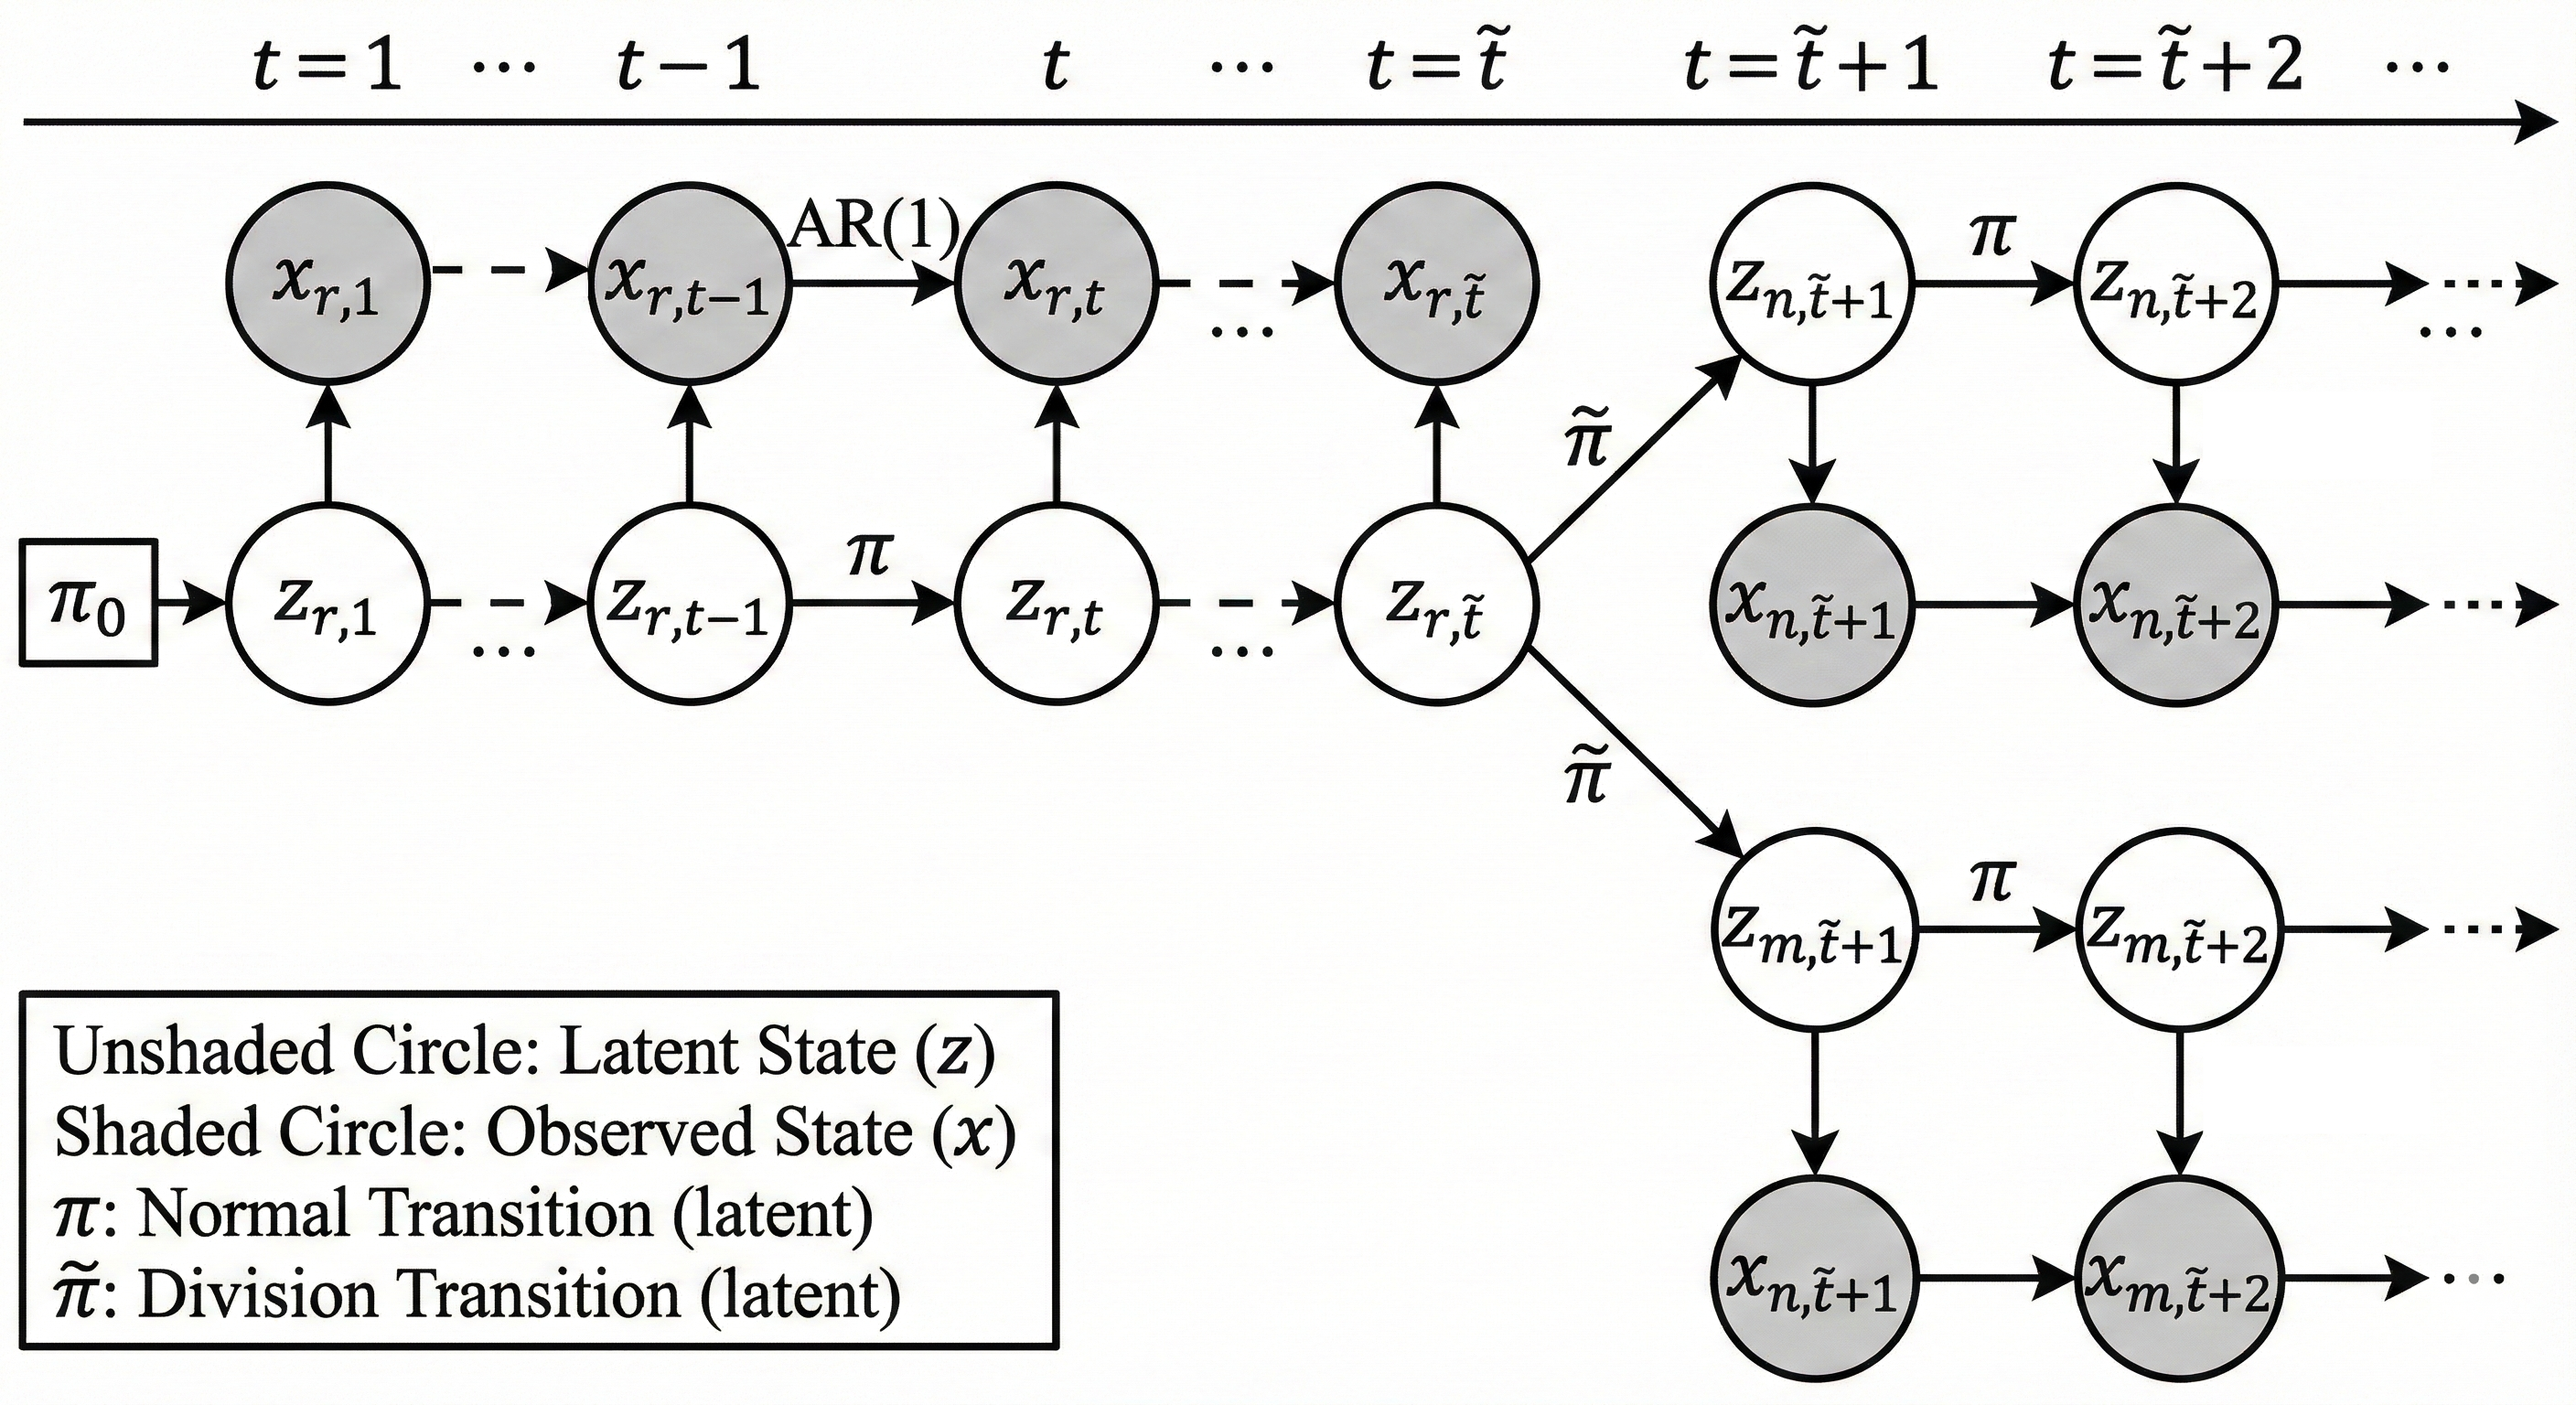
\includegraphics[width=0.8\textwidth]{figs/fig1.png}
        \caption{Tree AR-HMM Probabilistic model.}
        \label{fig:myfigure}
    \end{figure}

\section{Forward-Backward (E-step) Derivation}


\subsection{Forward Messages}
Initialize $\alpha_1^{(root}) = \pi \odot l_0^{(root)}.$ 
$$\alpha_{t+1}^{(c)} =\ell_{t+1}^{(c)} \odot \left[P_c^T \alpha_t^{(p)}\right].$$


\subsection{Backwards Messages}
Initialize for all cells at their "endpoint"- $\beta_t^{(c)} = \mathbf 1_k$
For a cell $r$ at time $t$, backwards message is given by:

$$\beta_t^{(r)} = \bigodot_{c\in C(r)} \left[P_c^T (\beta_{t+1}^{(c)} \odot \ell_{t+1}^{(c)} \right].$$

Here, if $C(r) = \{r\}$, then $P_c = P$. If $C(r) = \{n,m\}$, then $P_c = \tilde P$. 

That is, the backwards message is from the immediate children, and propagates up the tree so that $\beta_1^{(r)}$ includes the messages from all children. 


\subsection{Smoother Posteriors}

$$p(z_t^{(n)} | \text{All observations} ) \propto \alpha_t^{(n)} \odot \beta_t^{(n)}.$$


\subsection{Expected Transitions}


We need for each $(i,j)$, 
$$\xi_{ij} = \sum_t \sum_{n=1}^{C_{r,t}} \sum_{c_n \in [N_{n,t}]} \E_q \left[\Ind[z_{n,t} = i, z_{c_n, t+1} = j]\right] \Ind[n \to c_n \text{is not a division}]$$
and $\tilde \xi_{ij}$ for divisions. 
 
$$\E_q \left[\Ind[z_{n,t} = i, z_{c_n, t+1} = j]\right]  = \Pr( z_{n,t} = i, z_{c_n, t+1} = j) \propto  \frac{p(z_{c_n, t+1}=j | x_{1:T})}{p(z_{c_n, t+1}| x_{1:t})} P_{c_n}[i,j] p(z_{n,t} =i|x_{1:t}) $$


Step: 
\begin{enumerate}
	\item At time $t+1$
	\item For each cell, find its parent
	\item Calculate the above, masked for division events
	\item $carry \leftarrow carry + above $ 
\end{enumerate}
\subsection{Jax implementation} 
\section{M Step}




\end{document}
